\LUchapter{范畴论视角下的线性代数}

% 关于代数学的历史,最值得一读的文献大概是 J. Derbyshire 的 \emph{Unknown Quantity: A Real and Imaginary History of Algebra}.这本书的写作风格轻松明快,不难卒读,其中历数的历史,笔者在此不再赘述. 而由于现代代数学卷帙浩繁,难以尽数,而且其中的大部分主题也远超笔者心力之所能及,在这里,仅仅就一些主要趋势泛泛而谈,有识见的读者可以自行翻阅文献,不必为笔者为方便理解所作的简化以及本身不完整的理解所累.

% 按照笔者的思路,我们将首先正式引入范畴论.在范畴论的框架下,接下来我们要考虑的是代数与拓扑之间的联系,这会将我们引向两个截然不同的方向:同伦论(homotopy theory)和凝聚态数学(condensed mathematics).前者相较后者历史较为悠久,正好够我们历数从 1950s 到现代的一些发展;后者则方兴未艾,可供读者一窥当代数学家的风貌. 至于一些未被纳入此框架的探讨和研究,代数数论将作为最后的讨论的切入口.还有一些剩下的,例如群论、环论、表示论等主题的发展,则只能付之阙如了.

% 当然,还有一个被遗落的庞大的专题,就是在 Derbyshire 的书中开了个头的代数几何. 这一部分的探讨笔者无力完成,只能在此稍作提示——不过,在同伦论的部分中,我们也会见到其中的许多重要人物. 这个专题几乎是当代数学的前沿核心,但也正因为其核心地位,对它所作的任何不由杰出人物写下的讨论都显得有些不足,而且其研究所需的前置知识也远非本书所能及. 因此,在此我们只能无奈将其抛下,这并非轻视其重要性的表现.

这是本书的最后一章,也是最后一个未竟专题. 一切旅程都有终点,线性代数也不例外. 但是,终点同时也是一个起点,因此,在这里,我们将要引入现代数学中必不可少的一套语言——范畴论语言,并且使用这种方式来重述线性代数的一些概念,为本书画上一个句号. 可惜的是,因为篇幅有限,在这里不能重现利用范畴语言完成的全书所有内容的推导,但是我们会尽量走的远一些,同时也轻松一些. 在读者的代数基础尚且不算充足的时候,这一节的内容看起来可能有些抽象. 但如果在现代数学的路上走出更远,回头再来用这里的内容印证自己所学,相信读者依然会有所收获,这也就是未竟专题的未竟意义之所在.

在范畴语言引入之初,其提出者之一,Mac Lane 曾经下过一个断言. 他说,范畴论没有定理. 这是因为范畴论归根结底看起来只是一种“讲法”,正如我们在标题中所言,是一种“重述”,而非一套完全新颖的理论. 但是,这个断言很快就被打破了. 从本节会提及的 Yoneda 引理到本节不可能提及的 Freyd-Mitchell 嵌入定理,范畴论本身也逐渐发展成了一个生机勃勃的学科,并隐隐有成为数学基础的有力竞争者的趋势. 因此,最后,我们也希望读者思考,数学到底是什么?它是一种如范畴论所说,对对象和关系的研究,还是一种逻辑推导,抑或是一种直觉的形式化?如果读者在此方面有所意识,那么在未竟专题中走过的路也就都是有价值的.

\section{范畴、函子、自然变换}

范畴论的引入来自于 Samuel Eilenberg and Saunders Mac Lane \emph{General theory of natural transformations}, Trans. AMS, 58, p.p.: 231-294 (1945). 我们在此以现代的语言重述其概念,下面我们要呈现其中的三个核心定义:范畴、函子、自然变换.

\begin{definition}{}{}
    称以下资料为一个\term{范畴},记作 $\cC$:
    \begin{enumerate}
        \item 一族元素,每个元素称为其中的\term{对象},这一个族记作 $\Ob(\cC)$;我们将 $A \in \Ob(\cC)$ 简记作 $A \in \cC$;
        \item 一族 $A$ 到 $B$ 的箭头或者\term{态射} $\Hom_\cC (A, B)$,对于 $\Ob(\cC)$ 中的任意两个元素 $A, B \in \cC$,满足如下条件:
              \begin{enumerate}
                  \item 如果 $A, B, C \in \cC, \alpha \in \Hom_\cC (A, B), \beta \in \Hom_\cC (B, C)$,则存在复合 $\beta \circ \alpha \in \Hom_\cC(A, C)$;
                  \item 对于任意$D \in \cC, \gamma \in \Hom_\cC (C, D)$,都有\[
                            \gamma \circ (\beta \circ \alpha)= (\gamma \circ \beta) \circ \alpha;
                        \]
                  \item $\Hom_\cC (A, A)$ 中必有一个恒同元素,记作 $\id_A$,使得对于任意的$f \in \Hom_\cC (B, A)$,
                        \[\id_A \circ f = f \circ \id_B \]
              \end{enumerate}
    \end{enumerate}
\end{definition}

对这个定义,需要进行一些说明. 我们用“一族”的地方所指的未必是“一个集合”. 这是为了避免一些集合论上的麻烦,出现例如集合的集合之类的问题. 在范畴不会引起误会的情况下,我们将 $\Hom_\cC (A, B)$ 简记成 $\Hom (A, B)$,其中的元素 $f$ 也写成 $f\colon A \to B$ 或者 $A \stackrel{f}{\to} B$.

对于本书的读者而言,最熟悉的范畴无疑是线性空间的范畴. 准确地说,是域 $\F$ 上的有限维线性空间的范畴. 我们将其记作 $\FVect_\F$. 其中的对象就是所有的有限维线性空间,两个线性空间 $V, W$ 之间的态射 $\Hom (V, W) = \mathcal{L}(V, W)$. 另一个熟悉的范畴是 $\Set$,其中的对象就是所有集合,两个集合 $S, T$ 之间的态射就是从 $S$ 到 $T$ 的映射. 但是,出于习惯考量,当后面我们提及 $\Set$ 时,涉及的态射会变成从集合 $S$ 到 $T$ 的含入映射. 当然,范畴的对象并不总是这样“类似集合”的东西,虽然目前为止,这样理解已经足够了.

最后一个说明来自于结合律. 读者可能会认为,对于定义的第二条性质,最后的要求实属多余. 但实际上,如果我们只有抽象的点和箭头,很多性质也就无从谈起. 就像我们在学习线性空间的时候,它比起集合多了许多公理,因此也多了许多性质. 结合律实际上是范畴性质之根本,正如我们在下一个定义中会看到的一样.

\begin{definition}{}{}
    设 $\cC, \cD$ 为两个范畴. 称 $F$ 为 $\cC$ 到 $\cD$ 的一个\term{函子},如果:
    \begin{enumerate}
        \item 对 $\cC$ 中的每个对象 $A$ 它指派 $\cD$ 中的一个对象 $F(A)$;
        \item 对 $\Hom_\cC (A, B)$ 中的每个态射 $\alpha$ 它指派 $\Hom_\cD (F(A), F(B))$ 中的一个态射 $F(\alpha)$,满足
              \begin{enumerate}
                  \item 对于可复合的 $\alpha, \beta$ 都有 $F(\alpha \circ \beta) = F(\alpha) \circ F(\beta)$;
                  \item 对于任意 $A \in \cC$ 都有 $F(\id_A) = \id_{F(A)}$;
              \end{enumerate}
    \end{enumerate}
\end{definition}

最简单的函子的例子是一个范畴打到自身的恒同函子,它不会改变任何东西;以及 $\FVect_\F$ 到 $\Set$ 的忘却函子,它直接抛掉线性空间中的代数结构,只留下里面的元素. 现在我们考虑一个不那么平凡的例子:

\begin{example}{}{}
    考虑范畴 $\FSet$ 的对象是所有的有限集,其中的态射为含入映射. 则它到 $\FVect_\F$ 有一个显然的函子,是张成函子,我们将其记作 $\spa: \FSet \to \FVect_\F$. 它将一个有限集合映到由它张成的线性空间. 实际上,也就是将 $S = \{s_1, s_2,\ldots, s_n\}$ 映到一个形式和:

    \[
        \spa S = \left\{\sum_{i = 1}^n a_i s_i: a_i \in \F\right\}
    \]

    其上的线性空间运算都是显然的. 同样不难验证它将原来的含入映射映到一个线性映射,一个含入映射总是可以被对应到一个从子空间到原空间的嵌入.
\end{example}

另一个我们早就有所暗示的例子有点不同,它长得更加奇怪. 考虑一个范畴 $\cC$ 的对偶为将其中所有箭头反转的新范畴——不难验证它依然满足结合律,我们将其记作 $\cC^\mathrm{op}$,称为它的对偶范畴. 于是,我们发现,$\FVect_\F$ 到 $\FVect_\F^\mathrm{op}$ 有一个显然的函子,即对偶函子. 在对偶空间的部分中,我们已经验证了它满足函子的定义. 在较为古老的教科书中,这种打到对偶范畴的函子被称为反变函子,而上面定义的函子被称为共变函子,因为这类称呼已经淹没在历史的浪潮中了,所以我们也不会再使用了.

最后一个概念是最核心的,实际上也是范畴论被提出的初衷. 还记得上面提到的论文的标题吗?它叫做“自然变换的一般理论”,于是,下面我们就要说明,什么是自然变换. 这看起来可能会有点抽象:

\begin{definition}{}{}
    考虑两个函子 $F, G: \cC \to \cD$. 称这两个函子之间的\term{自然变换}是一族 $\cD$ 中的态射 $\theta = \{\theta_X\}$,其中 $X \in \cC, \theta_X: F(X) \to G(X)$,使得对于所有 $\cC$ 中的态射 $f$,下图交换:

    \begin{center}
        \begin{tikzcd}
            F(X) \rar["\theta_X"] \dar["F(f)", swap] & G(X) \dar["G(f)"] \\
            F(Y) \rar["\theta_Y", swap] & G(Y)
        \end{tikzcd}
    \end{center}

    通常,我们将其记成以下形式:

    \begin{center}
        \begin{tikzcd}
            \cC \rar[bend left=50, "F"{name=U}]
            \rar[bend right=50, "G"{name=D}, swap]
            & \cD
            \arrow[Rightarrow, from=U, to=D, shorten =2pt, pos=0.5, "\theta"]
        \end{tikzcd}
    \end{center}

    并将其称作\term{2-胞腔}. 在最后一节中,我们将重新讨论这个名词的含义.

\end{definition}

也许,我们应该采取一种更直观的看法来理解这一串概念,下面的一些概念来自于拓扑学,但并不严格,仅仅是提供一个比较方便的几何直观. 实际上,对拓扑和范畴论更加熟悉之后,读者会发现这个类比背后的深意.

\begin{figure}[htb]
    \centering
    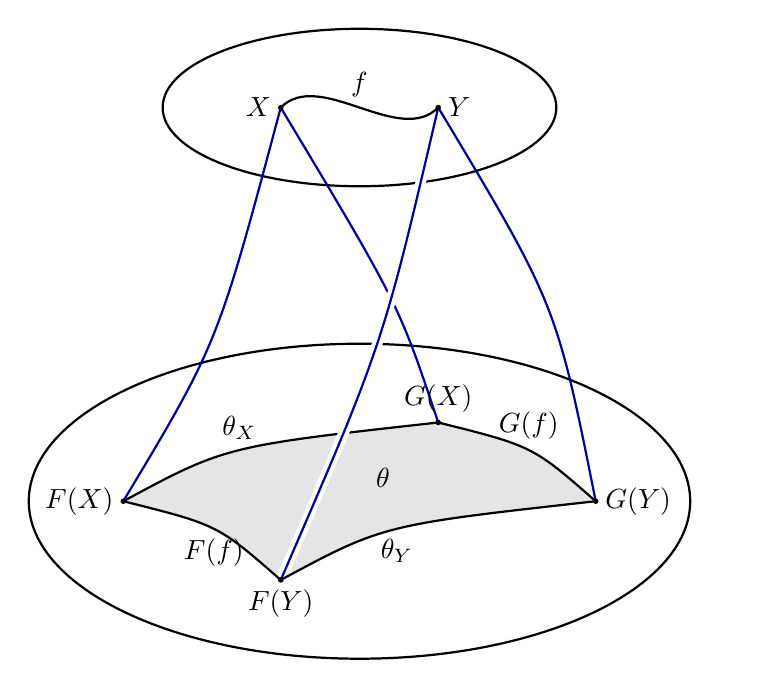
\begin{tikzpicture}
        \draw[thick] (0,3) ellipse (2.5 and 1)
        (0,-2) ellipse (4.2 and 2)
        node at (3, 3) {$\cC$}
        node at (4.7, -2) {$\cD$}
        coordinate (X) at (-1, 3)
        coordinate (Y) at (1, 3)
        coordinate (FX) at (-3, -2)
        coordinate (GY) at (3, -2)
        coordinate (GX) at (1, -1)
        coordinate (FY) at (-1, -3)
        coordinate (FX-GX-ct1) at (-1.7, -1.3)
        coordinate (FY-GY-ct1) at (0.3, -2.3)
        coordinate (FX-FY-ct1) at (-1.8, -2.3)
        coordinate (GX-GY-ct1) at (2.2, -1.3)
        coordinate (X-FX-ct1) at (-1.8, 0)
        coordinate (Y-FY-ct1) at (0.3, 0)
        coordinate (X-GX-ct1) at (0.5, 0.5)
        coordinate (Y-GY-ct1) at (2.5, 0.5);

        \fill[gray!20] (FX) .. controls (FX-GX-ct1) .. (GX) .. controls (GX-GY-ct1) .. (GY) .. controls (FY-GY-ct1) .. (FY) .. controls (FX-FY-ct1) .. (FX) -- cycle;

        \node at (0.3, -1.7) {$\theta$};

        \draw[thick] (FX) .. controls (FX-GX-ct1) .. node[above] {$\theta_X$} (GX) .. controls (GX-GY-ct1) .. node[above] {$G(f)$} (GY);
        \draw[thick,draw=blue!60!black] (X) .. controls (X-FX-ct1) .. (FX) (X) .. controls (X-GX-ct1) .. (GX);
        \draw[draw=white,double=blue!60!black,line width=1.5pt,double distance=0.8pt] (Y) .. controls (Y-FY-ct1) .. (FY);
        \draw[thick,draw=blue!60!black] (Y) .. controls (Y-GY-ct1) .. (GY);
        \draw[thick] (FX) .. controls (FX-FY-ct1) .. node[below] {$F(f)$} (FY) .. controls (FY-GY-ct1) .. node[below] {$\theta_Y$} (GY);
        \draw[thick] (X) .. controls (-.5, 3.5) and (.5, 2.5) .. node[above] {$f$} (Y);

        \node[left] at (X) {$X$};
        \node[right] at (Y) {$Y$};
        \node[left] at (FX) {$F(X)$};
        \node[right] at (GY) {$G(Y)$};
        \node[above] at (GX) {$G(X)$};
        \node[below] at (FY) {$F(Y)$};

        \foreach \point in {X, Y, FX, GX, GY, FY}
        \fill[black] (\point) circle (1pt);
    \end{tikzpicture}
    \caption{自然变换的几何直观}
    \label{fig:natural-transformation}
\end{figure}

首先,我们在一张纸上画两个面,表示两个范畴$\cC,\cD$. 在一个面上取两个点 $X, Y$,这是它上面的两个对象;然后,在另一个面上取四个点,分别表示 $F(X), F(Y), G(X), G(Y)$,即两个函子$F,G$在这两个点$X,Y$的取值. 注意,实际上两个函子分别是两个面之间的映射,如果把原像和像用线连接,展开来看的话,大概能看成是纸面上和纸面下的两张带有纹路的曲面. 然后,自然变换就是这两个曲面之间的连线$\theta$,对应到交换图上来,就是图中阴影区域的四条边. 实际上,我们的条件就是要求,这两族曲面$F, G$的结构和曲面之间的结构$\theta$都具备合适的连续性,如\autoref{fig:natural-transformation},这个东西在拓扑学中一般称为\term{同伦}.

在实践中,我们一般会称态射 $\theta_X$ 对于 $X$ 来说是自然的、典范的,或者说它满足函子性. 我们来看两个例子:

\begin{example}{}{}
    一个线性空间到某个商空间的投影映射. 考虑所有包含子空间 $U$ 的有限维线性空间. 显然,它们构成一个范畴,其间的态射定义为限制在 $U$ 上为恒同映射的线性映射,我们将这个东西记作 $\FVect_\F^U$.

    实际上,我们在说的是,考虑一个函子 $p\colon \FVect_\F^U \to \FVect_\F$ 将线性空间 $X$ 映到线性空间 $X/U$,另一个函子 $i\colon \FVect_\F^U \to \FVect_\F$ 将线性空间 $X$ 映到线性空间 $X$ 自身. 态射的映射都是显然的. 接下来,我们要表明存在一个自然变换 $\theta: i \to p$.

    现在,取任意的 $f\colon X \to Y$ 为 $\FVect_\F^U$ 中的态射,则我们需要使其交换的图表如下:

    \begin{center}
        \begin{tikzcd}
            X \rar["\theta_X"] \dar["f", swap] & X/U \dar["f/U"] \\
            Y \rar["\theta_Y", swap] & Y/U
        \end{tikzcd}
    \end{center}

    其中 $f/U$ 表示诱导的商映射,我们在不变子空间那一节中有所提及. 其中的 $\theta_X$ 和 $\theta_Y$ 就是我们通常称的典范投影,这也就是为什么这个投影被称为典范的.
\end{example}

下一个典范的结构我们也已经有所提及,它事关双对偶空间. 为了方便起见,对于函子 $F: \cC \to \cD$,我们记 $F^\mathrm{op}: \cC^\mathrm{op} \to \cD^\mathrm{op}$,它和原来的函子其实毫无差别,只有一点形式上的不同. 记对偶函子为 $-^*$,这是因为我们通常用 $V^*$ 表示对偶的空间,$f^*$ 表示对偶映射. 那么,我们就有 $(-^*)^\mathrm{op} \circ -^*$ 是典范同构. 这个事情的证明也是检查交换图,我们早已构造了这样的映射,也就是所谓的到双对偶空间的典范同构.

最后一个例子稍微有点特别,为了给出这个例子,我们需要定义一个与自然变换稍微有点不同的东西,强名之曰自然反变换\footnote{英文为 dinatural transformation,这个翻译稍微有点奇怪,但凑合用. }. 它的目标实际上是处理一些反变函子的情形,其它定义完全一致,不过它要求:$F: \cC \to \cD, G: \cC \to \cD^\mathrm{op}$,而它对应的交换图是:

\begin{center}
    \begin{tikzcd}
        F(X) \rar["\theta_X"] \dar["F(f)", swap] & G(X)\\
        F(Y) \rar["\theta_Y", swap] & G(Y) \uar["G(f)", swap]
    \end{tikzcd}
\end{center}

那么正如读者所料,我们要给出的结果就是:

\begin{example}{}{}
    不存在从一个线性空间到其对偶空间的非零自然反变换.

    现在,我们需要考虑下面的交换图:

    \begin{center}
        \begin{tikzcd}
            X \rar["\theta_X"] \dar["f", swap] & X^*\\
            Y \rar["\theta_Y", swap] & Y^* \uar["f^*", swap]
        \end{tikzcd}
    \end{center}

    我们知道,不管 $X$ 怎么取,总能取到一个 $f$ 使得 $f$ 将 $X$ 中的所有元素映到 $Y$ 中的零元,而参照我们的定义,这时的 $f^*$ 取值只有 $X^*$ 中的零元,因此,$\theta_X$ 为了让这个图交换,只能让所有元素映到零元.
\end{example}

可见在选取了合适的形式化方法之后,这些看上去无从下手的概念的证明变得无比单纯. 这实际上在表明,从一个空间到它的对偶空间不存在典范的同构.

\section{范畴论的构造}

单单是范畴、函子和自然变换显然什么都不能给出. 现在,我们无非是形式化了一些原来就已经说出的东西,顶多是最后对自然性的表述稍稍有些新意. 范畴论最核心的点实际上在于,它告诉了你很多被定义的东西实际上有其他的定义方式,这就是我们在这一节会讨论的内容.

\subsection{单态射、满态射和同构}

当我们在描述映射的时候,我们通常会讨论它是单的,满的,还是同构. 正如前面矩阵空间中关于指数映射的讨论中所表明的那样,这个性质实际上是非常不平凡的. 因此,这些性质应当在范畴论中得到恰当的推广——但是,时刻记住,现在我们的对象不同于以往我们做操作的集合,虽然我们还是能够从中汲取灵感.

先考虑集合的情况. 单射在我们看来,是如果像相同则原像相同,也就是说,每个原像集中的元素都有不同的像. 那么,就应当存在一个函数把它翻译回去,使得它在原像集上是恒同映射,也就是说:

\begin{lemma}{}{}
    考虑集合 $S, T$,一个函数 $f\colon T \to S$ 是单射当且仅当存在映射 $g\colon S \to T$ 使得 $g \circ f = \id_T$.
\end{lemma}

证明如上所述,形式化的写法留给读者,对偶地,我们就有:

\begin{lemma}{}{}
    $f\colon T \to S$ 是满射当且仅当存在映射 $g\colon S \to T$ 使得 $f \circ g = \id_S$.
\end{lemma}

而后面的这个定义是纯粹用箭头完成的,因此,它就能被推广到态射的情形:

\begin{definition}{}{}
    考虑范畴 $\cC$ 和其中的态射 $f\colon A \to B$.
    \begin{itemize}
        \item 称 $f$ 是\term{单态射},如果存在 $g\colon B \to A$ 使得 $g \circ f = \id_B$;
        \item 称 $f$ 是\term{满态射},如果存在 $g\colon B \to A$ 使得 $f \circ g = \id_A$;
        \item 称 $f$ 为\term{同构},如果存在 $g\colon B \to A$ 使得 $f \circ g = \id_A$ 且 $g \circ f = \id_B$;
        \item 如果 $A$ 和 $B$ 之间存在一个同构,则称 $A$ 和 $B$ 同构.
    \end{itemize}
\end{definition}

读者不难发现,恒同映射是一个同构. 这样的结构看上去就像一个逆元. 如果所有的态射都是同构,那么如果所有对象构成集合,态射也构成集合(这是为了避免一些集合论纷争),则我们将这个范畴构成一个\term{群胚}或者\term{广群}. 其态射集满足某种意义上的群结构. 实际上,在习题中我们会更进一步地发现相关的性质.

这里有一个麻烦的事情:同构一定既是单态射又是满态射,但既是单态射又是满态射的态射不一定是同构. 如果后者成立,则我们将这个范畴称为平衡范畴. 实际上,在通常的情形下,这个性质都是成立的.

\subsection{泛性质:始对象和终对象}

我们知道,一个范畴就是对象和箭头,那么,下面的定义看起来就很合乎情理:我们要选出箭头比较特殊的那些对象.

\begin{definition}{}{}
    称一个对象 $A \in \cC$ 为始对象,如果对于任意 $B \in \cC$ 都有 $|\Hom_\cC (A, B)| = 1$. 终对象是对偶范畴中的始对象. 如果一个对象既是始对象又是终对象,我们称其为零对象.
\end{definition}

注意,终对象的定义和始对象是完全对偶的,所以,很多时候我们其实不太区分这两种对象,它们具备的 $|\Hom_\cC (A, B)| = 1$ 的性质我们往往称为泛性质. 一般的,泛性质成立表明它实际上是一个定义性的东西:

\begin{theorem}{}{}
    所有始对象都是同构的、所有终对象都是同构的.
\end{theorem}

证明过于显然,留作读者练习. 重要的是例子:$\FVect$ 中,$\{1\}$ 是零对象. 这实际上说明了这个玩意的特殊性,但我们对它的特殊性早已习以为常. 剩下的一些例子我们会在后面的构造中一一给出——实际上,所有不太平凡的例子都要求我们构造一些更为奇特的范畴.

\subsection{Hom 函子和 Yoneda 引理}

注意到,如果 $\cC$ 和 $\cD$ 都是范畴,则 $\cC \times \cD$ 也是一个范畴,其上的对象和态射都是显然的. 我们首先考虑这样一个函子:
\[
    \Hom: \cC^\mathrm{op} \times \cC \to \Set
\]

它将对象 $(c, c')$ 映到它们之间的态射集 $\Hom_\cC(c, c')$,而将态射 $(f: c \leftarrow d, f': c' \to d')$ 映到一个 $\Hom_\cC(c, c') \to \Hom_\cC(d, d')$ 的映射,以复合的形式:
\[
    \Hom(f, f')(q: c \to c') = f' \circ q \circ f
\]

这个东西看起来乌七八糟的,但是在后面谈到张量积的时候,这个定义会体现出一个非常明显的性质. 在此,我们考虑另一种

\subsection{伴随函子}

\subsection{逗号范畴}

\subsection{和与积、极限和余极限}

\subsection{纤维化和余纤维化}

\section{幺半范畴及其性质}

\subsection{函子范畴和单子}

\subsection{Beck 单子化定理*}

\subsection{张量积}

\section{2-范畴一瞥}

\subsection{伴随和伴随}

\subsection{作为 2-极限的逗号范畴}

\subsection{走向无穷范畴:为什么我们需要套娃?}

\begin{exercise}
    \exquote[——《收获与播种》,格罗滕迪克]{每一门科学,当我们不是将它作为能力和统治力的工具,而是作为我们人类世代以来努力追求的对知识的冒险历程,不是别的,就是这样一种和谐,从一个时期到另一个时期,或多或少,巨大而又丰富:在不同的时代和世纪中,对于依次出现的不同的主题,它展现给我们微妙而精细的对应,仿佛来自虚空。}

    \begin{enumerate}  % 若不需要编号,则直接使用 enumerate 环境
        \item 证明以下两个态射的性质:
        \begin{enumerate}
            \item 如果 $A$ 与 $B$ 同构,那么 $A$ 与 $B$ 之间的同构映射是唯一的;
            \item 函子保持态射的单、满性质.
        \end{enumerate}
    \end{enumerate}
\end{exercise}
